\section{System}
\label{sec:system}

\Cref{fig:arch} shows the forward pipeline. Each stage combines proposal generation with deterministic checks;
the recovery controller can return a failed run to an earlier stage.

\begin{figure}[t]
\centering
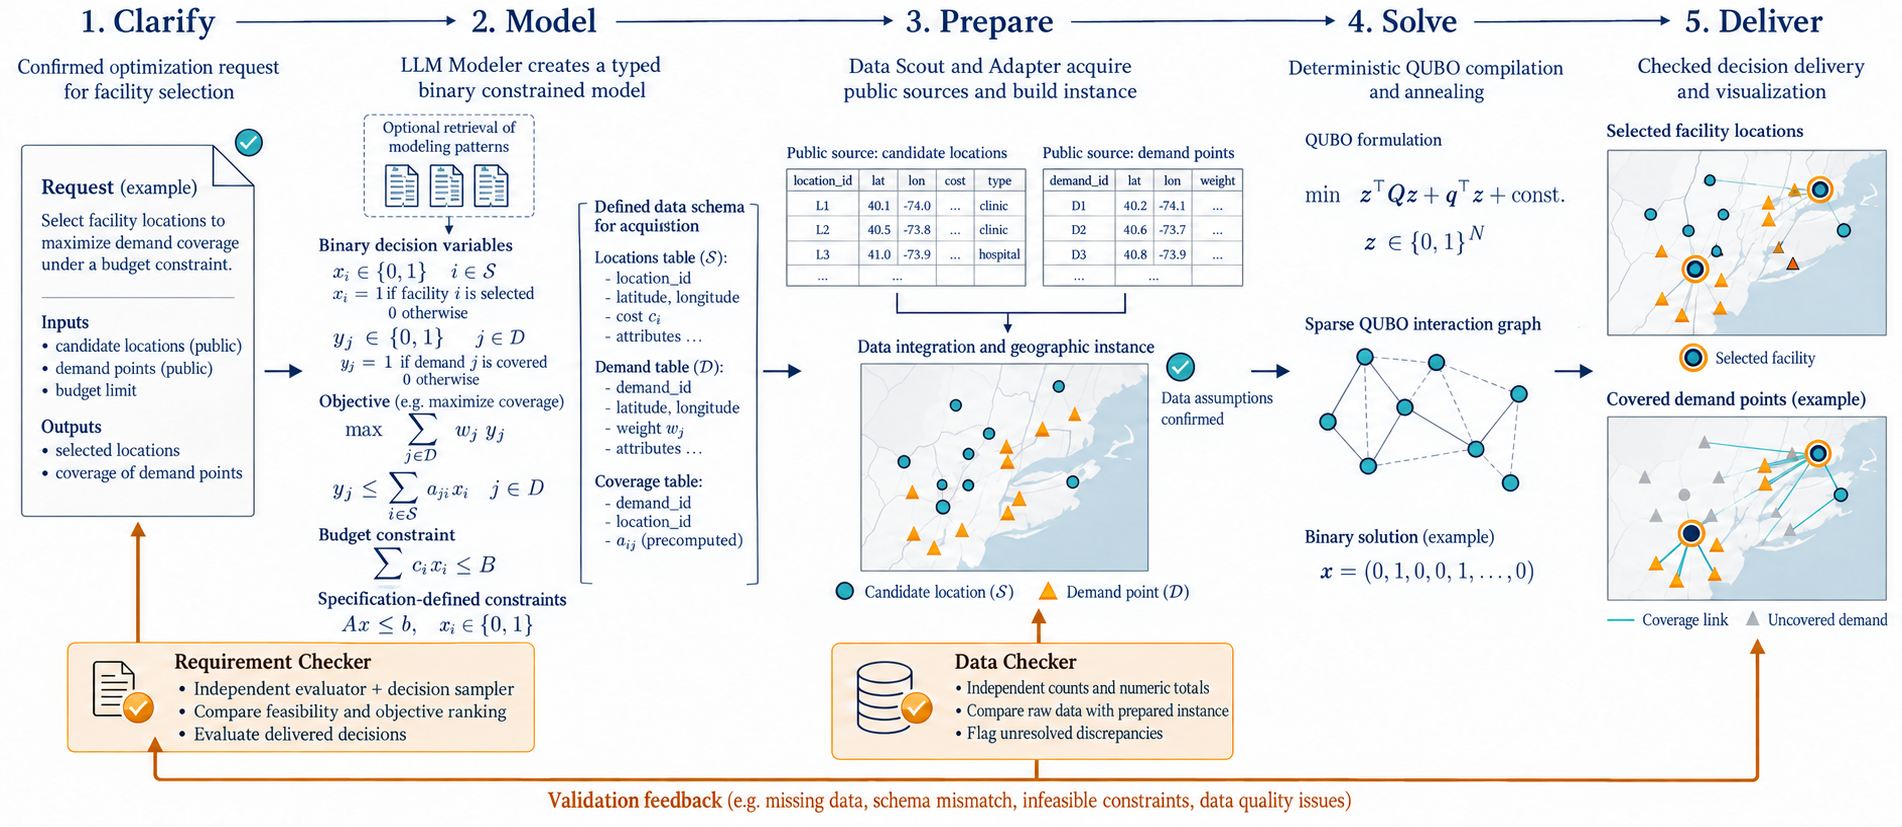
\includegraphics[width=\linewidth]{figures/skill/workflow-illustrated.png}
\caption{Illustrative end-to-end facility-selection workflow. A confirmed request becomes a typed binary
model and schema, a prepared public-data instance, a QUBO and a checked decision. Coverage variables prevent
double-counting; QUBO variables include decision and encoding auxiliaries. Checker evidence supports bounded
repairs, not a guarantee of correctness. Tables, coordinates, maps and bit assignments are schematic examples.}
\label{fig:arch}
\end{figure}

\subsection{Clarification}
The Clarification Agent drafts a specification (decision variables, objectives, hard and soft constraints, data
needs, a size estimate against the target backend) and asks at most five questions per round, each with options
and a suggested default; everything else it decides itself and records as an assumption that the user accepts or
corrects at confirmation. When the specification depends on external facts (laws, standards) it proposes up to
three search queries; code runs them, fetches the pages (including government sites and PDFs) and extracts the
passages relevant to the query, and the agent drafts again with the findings. Every claim taken from the web must
cite a page that was actually fetched: garbled URLs are corrected to the nearest fetched page and anything else is
marked unverified. Findings are stored with the session, so a rerun does not search again.

\subsection{Modeling}
The Modeling Agent writes a Python module: a data schema, a synthetic data generator, a builder that returns a
typed model over binary variables (linear and quadratic objective terms; linear, exclusion and implication
constraints), and a function that describes a solution. It also states its own modelling choice (e.g.\ an exact
formulation or an approximation that fits the target hardware). Code validates the module on a small instance by
brute force and with problem-independent checks, each of which was added after observing the failure it detects:
\begin{itemize}
  \item the data survives a JSON round trip (the model is later fed stored data);
  \item the objective is not empty;
  \item no hard constraint's squared penalty is folded into the objective (detected as uniform couplings over the
        constraint's variables);
  \item hard constraints of the specification are not all missing from the model;
  \item the model is not solvable by sorting, i.e.\ it does not consist of a linear objective with
        non-overlapping ``choose $k$'' constraints, unless the agent declares and justifies it;
  \item the small instance is feasible, with a hint when a parameter is not scaled to the instance size.
\end{itemize}
Retries show the agent its previous module and the errors and ask for a repair rather than a rewrite. Drawing is
split into a separate short task: a Visualizer writes a function that returns a figure \emph{specification} in one
of five fixed formats (map, schedule, routes, graph, selection), which code validates and renders.

\subsection{Data acquisition and preprocessing}
A Data Scout turns the model's data schema into searches on open-data platforms and OpenStreetMap, and screens
candidates for relevance and readability. Connectors support CKAN, Socrata, Opendatasoft, ArcGIS Hub and the
European data portal; supported WFS layers are requested as JSON in WGS84. These connectors use links returned
by catalog APIs or fetched source pages. Their implementation does not establish reliable coverage of every
portal or data format. The user can select sources manually, or a bounded acquisition
controller tries existing readable tables and then alternative sources. Download and conversion failures are
recorded; a retry receives the preceding errors rather than repeating the same request blindly. Unresolved
data gaps and assumptions are surfaced for confirmation. A Data Adapter maps the tables to
the model's schema. It never reads raw data: it sees bounded profiles of each table (columns, types, ranges,
missing values, a few rows) and writes code that runs on the full tables, preferably by calling a tested
preprocessing toolkit for situations that recur in public data: encodings (Big5, UTF-8 with BOM), Shapefiles and
GeoJSON, total and subtotal rows, rows split by category, stacked periods, mixed administrative levels, ROC
calendar dates, numbers stored as text, coordinate systems (via EPSG codes), variant characters in place names,
geocoding with explicit precision levels, road distance and time matrices, and size reduction by weighted
clustering. Every step is written to a provenance record (sources, licences, row counts, match rates) that the
user can inspect before approving data assumptions. Unknown licences remain marked as unknown. The adapter's
output is checked on the full data against the declared interface and example input.

\paragraph{Typed data interface and administrative joins.}
The current \texttt{DATA\_SCHEMA} separates entity sets from parameters indexed by those sets. It declares
source class, type, unit, derivation and, where available, period, geography and granularity. Checks reject
unknown fields, duplicate entity IDs, incompatible dense-array shapes, invalid sparse indices and invalid
numeric values. Canonical spatial inputs use WGS84 latitude and longitude, and distance parameters use metres.
Derived fields can require specific toolkit calls. For mixed administrative levels, the toolkit can propagate a
parent district before filtering village rows, then join on district and village together; duplicate keys and
unmatched rows are reported. These checks address common loss and misalignment mechanisms, but declared units
and correctly shaped arrays can still encode the wrong interpretation.

\paragraph{Independent data computation.}
When enabled, a Data Checker receives the confirmed request, schema and raw-table profiles, but not the Adapter
code. It writes a separate computation of expected entity counts and numeric totals. Code compares these with
the prepared instance, using a 0.5\% total tolerance with a unit-scale floor. Counts are skipped for sets declared
reducible. Disagreements trigger bounded Adapter feedback; a remaining disagreement is marked for review.
Checker-generation failures are recorded. This optional mechanism is enabled in the checker arms of the batch
protocol, not universally in every acquisition call. Aggregate agreement cannot detect every wrong join,
per-entity permutation or shared misunderstanding by the two LLM roles.

\paragraph{Acquisition safeguards.}
Several problem-independent rules come from failures in development runs. Candidates are screened by a
preview of their first bytes (column names and a first record) as well as by title, and raw record tables are
preferred over reports and documentation. A candidate is relevant if it supplies at least one required item, since
sources are joined later; boundary maps count as sources of coordinates. When one dataset holds several period
files, code keeps only the latest; when the request names a publisher, that publisher's data take precedence over
crowd-sourced points. The loader extracts record lists nested in JSON responses, recognizes web pages saved
under data names, tolerates isolated malformed rows (and reports them), skips title lines above a header, and
streams large files to disk. Coordinates stored as text are inspected for projected systems, and $(0,0)$
coordinates are rejected as missing values. When a join on names finds duplicate keys and both tables carry a
parent level, the join adds that level itself; otherwise the flag explains how to recover the parent level.

\paragraph{Requirement Checker and decision identities.}
\Cref{fig:verificationlayers} separates the runtime checker roles from the external evaluation judge.
A separate Checker generates an evaluator and decision sampler from the confirmed specification and data
schema without seeing the model formulation. Model variables carry \texttt{variable\_keys} that identify their
underlying decisions independently of bit positions. Before solving, sampled decisions are evaluated both by
the Checker and by the model with decision variables fixed; a time-limited MILP optimizes remaining helper
variables where supported. Tests compare feasibility, objective ranking and rejection of perturbed decisions.
After solving, the Checker evaluates the delivered decisions. Timeouts and unsupported helper interactions
remain inconclusive, and so do sampled decisions that have no model variable (a model may fix some decisions to
break symmetry, e.g.\ the first stop of a closed tour). The Checker computes distances with the same tested
toolkit as the Adapter and must not require what the specification leaves free. A disagreement supplies repair evidence; because the Checker is also LLM-generated,
agreement is not a proof of semantic correctness. The acceptance judge in \cref{sec:autonomousprotocol} is
separate from this runtime role.

\begin{figure}[tbp]
\centering
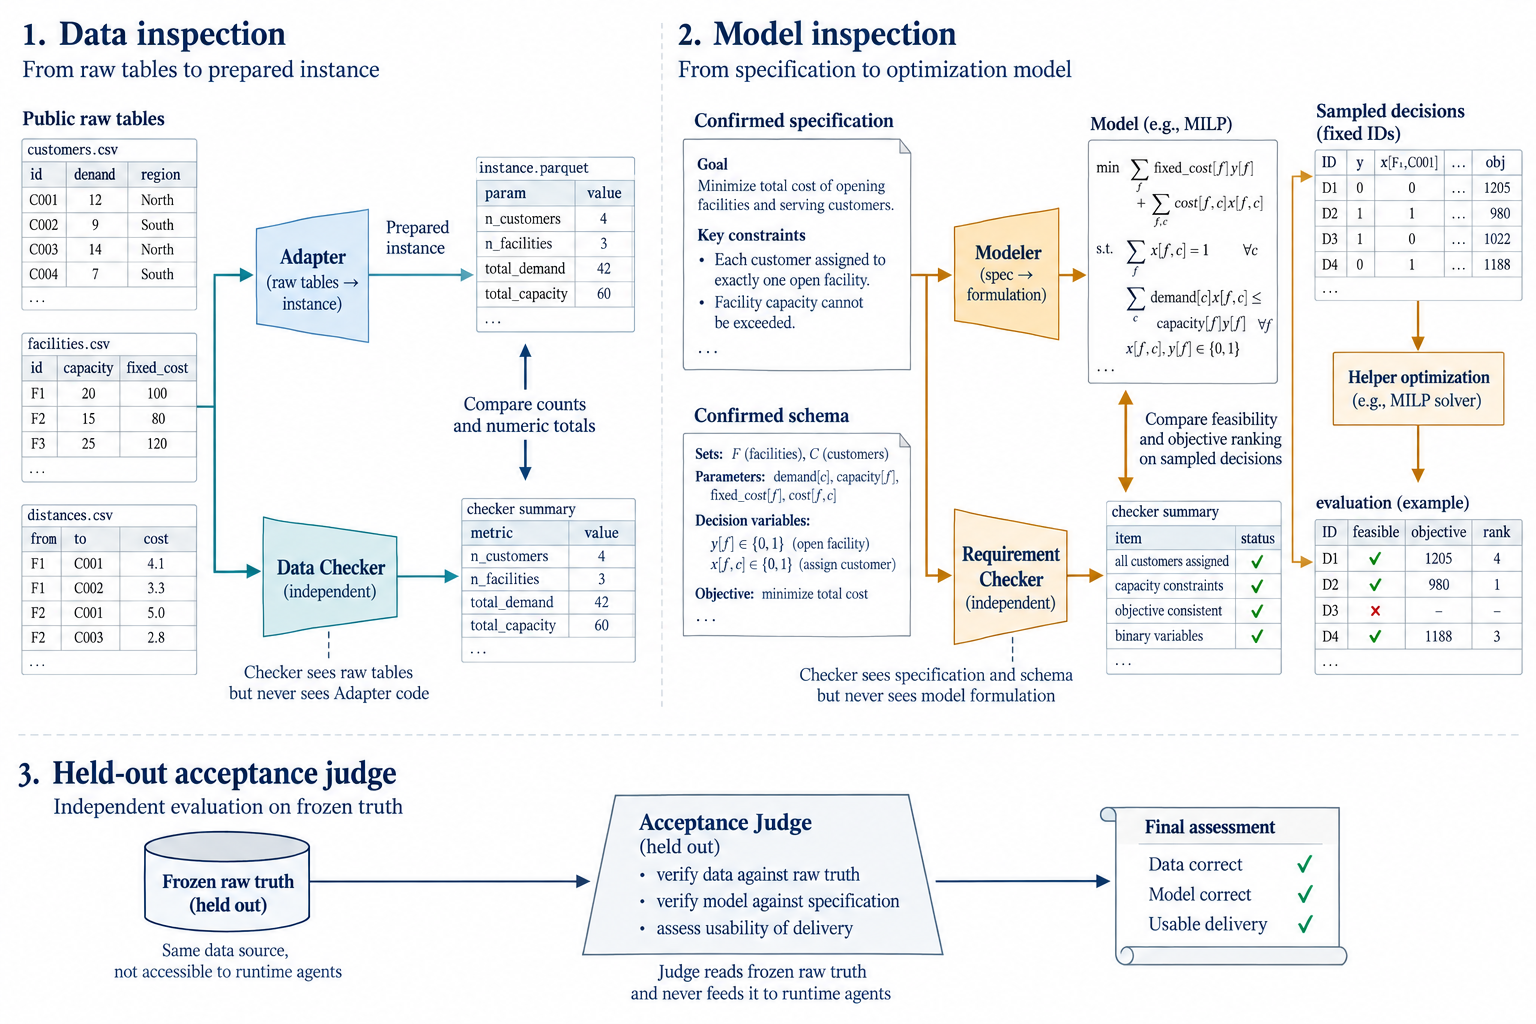
\includegraphics[width=\linewidth]{figures/skill/verification-reference.png}
\caption{Illustrative data inspection, requirement inspection and external acceptance judging. Tables,
formulations, evaluation values and check marks are schematic examples, not experimental results.
Agents receive bounded raw-table profiles and write code that operates on full tables; the Requirement
Checker does not see the formulation. Helper optimization is used where supported. Checker agreement is
evidence rather than a correctness guarantee; held-out judge truth is not supplied to runtime agents.}
\label{fig:verificationlayers}
\end{figure}


\paragraph{Optional retrieval of modelling patterns.}
The Modeling Agent can select up to three general patterns by title from a local knowledge library and receive
their text in its modelling prompt. Repairs reuse the selected pattern IDs. This is a bounded retrieval step,
not a pretrained change to the LLM or an embedding-based search service. The pattern-retrieval arm tests its
incremental effect; the earlier tuning-knowledge experiment addresses a different stage.

\subsection{Encodings, guardrails and the tuning loop}
Constraints are compiled to QUBO penalties through an encoding library (squared penalties for equalities, binary
or unary slack and unbalanced penalization~\citep{montanez2024unbalanced} for inequalities, pairwise penalties for
exclusions and implications), each verified in both directions on small cases. A tuning loop proposes penalty
weights, encodings and solver parameters, runs the backend, extracts backend-independent feedback (feasibility,
violation rates per constraint, objective, gap, energy spread, backend-specific signals such as chain breaks) and
proposes the next configuration. Guardrails reject weights below the single-flip lower bound for exact
encodings~\citep{verma2020penalty}, unbalanced penalties whose reward on feasible points exceeds the objective's
range, out-of-range solver parameters and anything beyond the hardware budget. On large models agents see
constraint \emph{families} (names with numbers abstracted) instead of individual constraints, which bounds prompt
size by the number of constraint kinds rather than by the instance size. The single-flip floor is a heuristic
guardrail, not a general proof of global-optimum preservation. Results are ranked by original-problem
feasibility and objective; QUBO energy is diagnostic because changing penalties changes its meaning.

\paragraph{Parameterized compilation and diagnostics.}
For each encoding combination, the compiler assembles the objective and unit-weight penalties in PyQUBO and
compiles once~\citep{pyquboDocs}. Subsequent rounds substitute named penalty placeholders. Explicit variable
labels preserve the original decision and slack indices. Labelled penalties help diagnose a selected sample,
but do not replace original-constraint checks: a feasible decision may have incorrectly filled slack variables
and hence a nonzero encoded penalty. Approximate unbalanced penalties are excluded from zero-penalty
constraint diagnostics.

\paragraph{Penalty-only search policies.}
The UI selects \texttt{default} initially; penalty-search policies remain explicit alternatives.
Alongside the existing agent, rule, random and joint Optuna policies, four policies vary penalties while
keeping solver effort at its capped defaults. Optuna TPE uses two startup trials; its score assigns every
feasible result a higher value than an infeasible result, then reflects the original objective. Grid search
enumerates a bounded logarithmic grid lazily. Cross-entropy search updates a log-weight distribution from
elite rounds ranked by original-problem quality, with a variance floor and bounded sampling attempts.
A sequential controller doubles penalties of violated constraints up to a configured ceiling. The grid and
cross-entropy designs draw on QHyper~\citep{qhyperDocs}, while sequential control, feasible-round stopping
and checkpointing draw on Kaiwu~\citep{kaiwuDocs}; these are local adaptations, not SDK calls.
All policies share the backend interface, guardrails and solver-call budget.

\paragraph{Stopping and checkpoint recovery.}
The controller can optionally stop after a configured number of rounds containing a feasible solution; this
condition is disabled by default and does not certify quality. After each completed round it saves the typed
model, settings, feedback, feasible penalty configurations and cumulative call count. The four penalty-only
policies reconstruct their search state from this history. Resume checks the model, backend, policy, seeds and
settings, while allowing an increase in the total call budget. A pending marker is written before submission;
if an interruption leaves a call unresolved, automatic resubmission is refused until the backend record is
inspected. This does not provide an exactly-once transaction at an external solver.

\subsection{Recovery across data, modelling and solving}
\label{sec:recovery}
\Cref{fig:recoveryroutes} summarizes the evidence used to route a run through checking, repair and delivery.
Before annealing, the controller checks basic data and constraint consistency and runs a time-limited HiGHS
feasibility check. Proven infeasibility is reported without an annealer call; timeout remains unknown and
does not imply that the problem has no solution. A feasible conventional solution supplies a quality baseline.
For quadratic objectives, the baseline combines a feasible point with bounded local improvement; it is not
labelled an optimum. Only a certified optimum of the linear model is used as an exact reference.

Before solving, a bounded repair callback can regenerate the model when acquisition reports a schema mismatch,
then rerun preparation against the new interface. Source-download failures and arbitrary Adapter exceptions do
not automatically imply a modelling fault. Workflow callbacks can subsequently use data or requirement-check
evidence to propose a revised Adapter or model.

Solver failure alone does not justify changing the model. Evidence of a formulation error can route the run
back to modelling; data mismatches route it to preparation, and unresolved resource shortfalls return a
diagnosis to the user. Repairs are bounded and share the remaining solver-call budget. A replacement is
validated before becoming active. A requirement map checks coverage of every confirmed hard requirement; a requirement guaranteed by the variable
design itself (e.g.\ a single closed tour under position encoding) is mapped with a stated justification and is
still tested by the Requirement Checker and the judge. Clarification records what must hold, not modelling
techniques.
Code repairs are compared on the same original data: changes to existing constraint formulas, bounds or
objective coefficients require confirmation. Fixed user inputs are protected against data-level changes.
Explicit data contracts check declared units, periods, scope, granularity and source correspondence;
unknown metadata remains a review item. These checks cannot prove that a repair preserves the natural-language
specification or that declared data semantics are true.

Model code, data and provenance are stored together in immutable versions with an atomic active pointer.
A durable task record states the current stage and next action. Prepared-data caches require matching code,
specification, notes and file hashes; the UI can resume supported solver checkpoints.
Generated model and adapter code runs in separate processes with timeouts, limiting hangs and crashes; this
is process isolation rather than a security sandbox. Results are tied to the version that produced them.
Delivery distinguishes usable solutions, solutions with limited quality, and absence of a usable solution.
If the annealer produces no feasible solution or trails the validated baseline beyond the configured
tolerance, the baseline can be delivered with its source stated. A Checker objection after solving triggers a
model repair only while solver calls remain to solve the repaired version; otherwise the solution is delivered
with the objection as a warning, and a repaired version left unsolved falls back to the earlier version's
annealer result. Figure or explanation failure does not
discard the saved solution.

\begin{figure}[tbp]
\centering
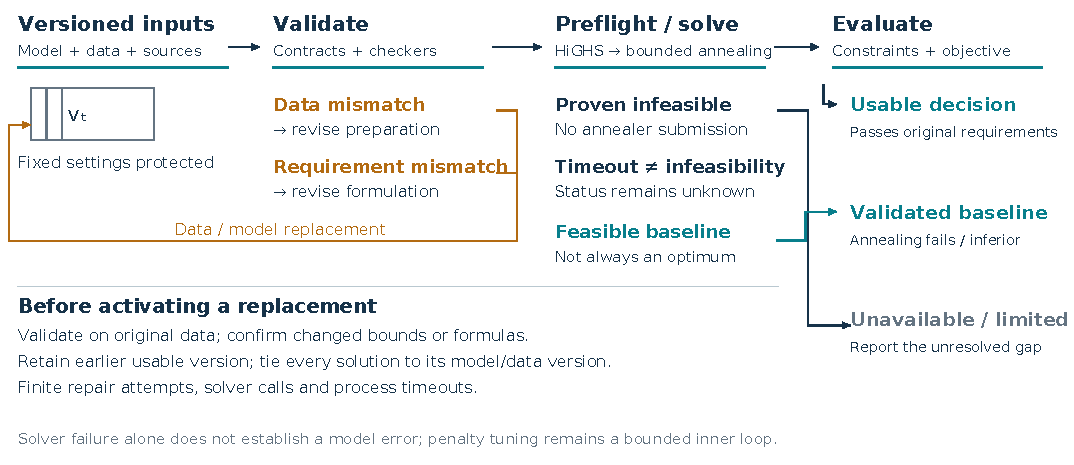
\includegraphics[width=\linewidth]{figures/skill/recovery-routes.pdf}
\caption{Evidence routes failures to the relevant stage. A repaired version must pass checks before activation.
Proven infeasibility avoids an annealer submission; a timed-out preflight does not prove infeasibility.
A validated baseline may be delivered when annealing fails or trails it. Repairs and solver calls are bounded.}
\label{fig:recoveryroutes}
\end{figure}


\subsection{Backends and serving}
The same QUBO can be submitted to simulated annealing (dwave-samplers), a GPU annealer (Compal GPU Annealer 2.0,
cloud service), the Fujitsu Digital Annealer v3c~\citep{aramon2019digital} and D-Wave (Advantage QPU or the Leap
Hybrid BQM service), with energies recomputed locally so results are comparable across backends. Our experiments
use simulated annealing, the GPU annealer and Leap Hybrid; a Digital Annealer submission was rejected at the
account's monthly usage limit, and no direct-QPU results are reported. All agents use Qwen3.6-35B-A3B (FP8)~\citep{qwen3report2025}
served by vLLM~\citep{kwon2023vllm} on NVIDIA L40S GPUs; each call has a reasoning budget, and an answer that
exhausts it is retried once without reasoning.
